\section{Einleitung}


\subsection{Management Summary}


Geschäftsprozessmodellierung verleiht einem Unternehmen die Fähigkeit seine
Geschäftsprozesse so umsetzten dass sie:

\begin{itemize}
\item einfach nachvollziehbar sind
\item sich selbst dokumentieren
\item vollständig oder Teilweise automatisiert ablaufbar sind
\item einfacher mit der Unternehmens-IT zu verknüpfen sind
\end{itemize}

Diese Fakten führten dazu dass sich die Prozessmodellierung bereits in fast
allen Unternehmen durchgesetzt hat.
Unter dem vielfältigen Angebot an Notationen hat sich hierbei BPMN besonders
herrauskristalisiert.\\

Der Modellierung erfolgt in der Regel mit einer Software. Dabei gibt es eine
Vielzahl von Anbietern und Produkten zwischen denen es sich zu entscheiden gilt.


\subsection{Motivation}

\begin{quote}
"`Prozessorientierung ist seit Beginn der 90er Jahre als eine unverzichtbare
Maxime der Unternehmensgestaltung akzeptiert. In den letzten Jahren
haben viele Unternehmen Maßnahmen
 zur verstärkten Ausrichtung an ihren Geschäftsprozessen initiiert."'
\footcite[S.182]{prozessmanagement:leitfaden}
\end{quote}


Aussagen wie diese, zeigen dass die Prozessorientierte
Geschäftsprozessmodellierung mittlerweile fest in allen Unternehmen angekommen
ist.
Umso wichtiger ist es also, die Unterschiede und Feinheiten verschiedener Tools,
Prozesse und Anwendungsszenarien zu kennen.

\subsection{Ziel der Arbeit}

Die vorliegende Arbeit soll dem Leser einen vollständigen Überblick über die
Kernbereiche der Prozessmodellierung geben. Hierzu wird zunächst auf die
Entstehung und Notwendigkeit der Prozessorientierung eingegangen. Anschließend
sollen Vertiefungen der Methodik ein genaueres Verständnis erzeugen woraufhin
einige bekannte Software-Tools präsentiert werden.

\clearpage
\section{Geschäftsprozesse}

\subsection{Prozess}


Ein „Prozess“, vom lateinischen „processus“ („Fortgang, Fortschreiten“) ist von
der Wiederholung bereits existierender Vorgänge geprägt.

Es handelt sich dabei also um eine sich äufig wiederholte, eher sequentielle
Verkettung von Aktivitäten, wobei die Ausgangslage sowie das
angestrebte Ergebnis definiert und die erforderlichen Maßnahmen
kategorisiert bzw. spezifiziert sind. Dabei besetehen stets nur
unbedeutende Unsicherheiten in der Zielerreichung zum Beispiel "`Beschaffung
eines Zulieferteils"'.

\subsection{Definition und Management von Geschäftsprozessen}


Ein Geschäftsprozess besteht aus der wiederkehrenden Abfolge von logischen,
zeitlich zusammengehörigen und inhaltlich abgeschlossenen Aktivitäten, dessen
Durchführung als Ziel die Wünsche der Kunden, die ein Unternehmen besitzt, zu befriedigen trägt.
Eine höhere Kundenzufriedenheit bedeutet ebenfalls eine höhere Wertschöpfung.
Mit einem bestimmten Input und bestimmtem Ressourceneinsatz,
entsteht ein Output, der an einen Empfänger geht.
Dieser Empfänger kann ein Kunde, ein Lieferant oder eine innerbetriebliche Stelle sein.
Handelt es sich tatsächlich um einen innerbetrieblichen Prozess,
so kann davon ausgegangen werden, dass dieser organisatorisch dauerhaft geregelt wird.
\footcite[Vgl.][ ]{prozess:db}\\



Zusätzlich wird unterschieden zwischen Leistungs-, Unterstützungs- und
Führungsprozessen den sogenannten Prozessarten. Prozesse werden analysiert,
woraus eine Bewertung ihrer Funktionalität und Effektivität entsteht.
Ziel der Prozessanalyse ist vor allem die Schaffung einer Transparenz als
Voraussetzung für eine bestmögliche Prozesssteuerung, dem „Geschäftsprozessmanagement“.
Eine einfache Wortanalyse ergibt, dass sich das Geschäftsprozessmanagement
mit der Verwaltung von Geschäftsprozessen beschäftigt.
\footcite[S.13]{lehmann}\\

Dazu zählen insbesondere folgende Aspekte:
Identifikation, Planung, Dokumentation,  Gewichtung, Verbesserung,
Steuerung, Kontrolle und Organisation von Geschäftsprozessen.
Zusammengefasst ist das Hauptziel und damit allgemeine Anforderung in Unternehmen,
alle Prozessaktivitäten und Prozesse möglichst effizient auszuführen.
Die Herausforderung für Unternehmen besteht darin, dass diese
möglichst unterbrechungs- und fehlerfrei ablaufen.\\

Wenn die Prozesse und Unterprozesse einmal identifiziert worden sind,
erfolgt die Beachtung der oben genannten Aspekte in Form einer Modellierung.
Ein Prozessmodell dient dazu die kombinierte, überschneidungsfreie
und lückenlose Struktur zusammenhängender Prozesse in einem Unternehmen darzustellen.
Hierzu gibt es verschiedene Möglichkeiten.
Im einfachsten Fall werden textuelle oder tabellarische Beschreibungen verwendet.
Häufig werden Präsentations- oder Grafikprogramme genutzt, um einfache Ablaufdiagramme
zu erstellen. Sie bestehen meist aus Kästchen und Pfeilen, wobei keiner
bestimmten Methodik gefolgt wird.\\
Zur genauen Darstellung komplexerer Prozesse mit allen relevanten Aspekten,
wie Verzweigungsregeln,
Ereignissen, ausführenden Organisationseinheiten, Datenflüssen usw.,
genügt eine grobe Modellierung nicht. Hierfür werden geeignete Notationen benötigt.
Mit welchen Symbolen die verschiedenen Elemente von Prozessen dargestellt werden,
was sie genau bedeuten und wie sie miteinander kombiniert werden können,
wird durch die Notation festgelegt. (Prozessmodellierung)
Welche Merkmale in Prozessmodellen abgebildet werden, hängt vom
Modellierungszweck und der verwendeten Modellierungssprache ab.
Die Regeln zur Modellierung von Geschäftsprozessen werden in folgenden Kapiteln deutlich.

\clearpage
\section{Prozessmodellierung und Notationen}

Im Zuge der Modellierung hat man es mit Zeichen unterschiedlichster Art zu tun.
Prozessmodelle können in Form von Texten, Tabellen oder Grafiken dargestellt werden.
Üblicherweise wird eine Modellierungssprache verwendet,
die eine Notation zur Abbildung von Geschäftsprozessen zur Verfügung stellt.
In dieser Arbeit wird insbesondere mit der Notation BPMN gearbeitet.

\subsection{Ereignisgesteuerte Prozesskette}

EPK ist als Abkürzung einer ereignisgesteuerten Prozesskette zu verstehen und
ist für die detaillierte Modellierung und Veranschaulichung
von Geschäftsprozessen und Prozesselementen gut
geeignet.\footcite[Vgl.][]{lehmann}


Diese Notationsform ist 1992 unter der Leitung von
Scheer\footcite[Vgl.][]{scheer} entwickelt worden, somit wird die Bezeichnung
Sheer-Notation oft verwendet.
EPKs sind das Hauptdarstellungsmittel in Architecture of Integrated
Information Systems (ARIS), darunter Ereignisse,
Funktionen und Verknüpfungsoperatoren. Es gibt ebenfalls eine erweiterte EPK,
die weitere Merkmale, wie bspw. Organisationseinheiten, Rollen von Mitarbeitern,
sowie Datenbestände bzw. Informationssysteme, bietet.
Da die Entwicklung und Pflege sehr umfangreich werden können ist die
Nutzung von Softwarewerkzeugen notwendig.
ARIS unterstützt Unternehmen bei der Modellierung, Analyse und Optimierung von Prozessen.
Das Grundproblem, nämlich der steigende Wettbewerbsdruck bezüglich der Zeit,
Kosten und Qualität verlangt effiziente und effektive Organisationsformen.
Unter einer Prozessorganisation ist nun eine Organisationsform zu verstehen,
bei der die Strukturierung von organisatorischen Einheiten,
insbesondere  Prozessteams bzw. Funktionsbereiche,
den Kern- und Unterstützungsprozessen folgt.

\subsection{Business Process Model and Notation}

\begin{quote}
"`BPMN ist ein Standard und soll die Brücke zwischen Business und IT schlagen."'
\footcite[Vgl.][]{praxishandbuch:bpmn2}
\end{quote}

Business Process Model and Notation (BPMN) ist eine grafische
Spezifikationssprache in der Wirtschaftsinformatik und im Prozessmanagement.
\footcite[Vgl.][]{allweyer}

Es ist der Standard für graphische und XML-basierte
Geschäftsprozessmodellierung.
Mit seinen Symbolen und Elementen ist eine einheitliche, standardisierte Sprache,
Darstellung und Analyse der Prozesse möglich.
Im Gegensatz zu EPK könnte man BPMN als eine „junge Modellierungsnotation“ bezeichnen.
Sie wurde von dem IBM-Mitarbeiter Stephen A. White im Jahr 2002 entworfen,
daraufhin von der Business Process Management (BPM)
Initiative veröffentlicht und im Jahr 2005 an die Object Management Group (OMG)
zu einem Modellierungsstandard erklärt.

Um BPMN verstehen zu können, muss zunächst das Verständnis für BPM geschaffen
werden. BPM ist ein systematischer Ansatz, der
dazu dient sowohl automatisierte als auch nicht-automatisierte
Prozesse zu erfassen, zu gestalten und auszuführen.
Stattdessen wird häufig auch der Begriff Geschäftsprozessmanagement dafür
verwendet.\footcite[S.1]{praxishandbuch:bpmn2}

Mit Hilfe von BPM können Prozesse auf die Unternehmensstrategie abgestimmt werden,
sodass sich die Gesamtunternehmensleistung verbessert, sobald Prozesse innerhalb
einzelner Organisationseinheiten, unternehmensweit oder sogar unternehmensübergreifend
optimiert werden.

Zunehmend werden für die Ausführung von Prozessen Business Process Management-
Systeme (BPMS) eingesetzt. Ein BPMS enthält eine Process Engine,
die die Abläufe direkt anhand geeigneter Prozessmodelle oder
formaler Prozessbeschreibungen steuert.
Hierfür müssen die Modelle besonders strikten Anforderungen genügen,
da sie nicht von Menschen in ein Computerprogramm umgesetzt,
sondern direkt von einer Maschine abgearbeitet werden.

In Abhängigkeit von der Situation, den Ansprüchen und Zielen der einzelnen
Unternehmen ergeben sich vielfältige Nutzenpotenziale
durch die Anwendung von BPMN. Es wird die verständliche Definition
und Dokumentation von Prozessen für die tägliche Anwendung und zur
Orientierung von Managern und Mitarbeitern geschaffen.
Zudem werden das Modell und die Notation standardisiert und stellen eine
gleiche Interpretation der gegebenen Prozessdefinition
von allen Prozessbeteiligten sicher. Verbesserung der Zusammenarbeit
zwischen Fachabteilung und IT-Dienstleister durch eine
anschauliche graphische Prozessmodellierung einerseits und eine präzise
Prozessdarstellung entsprechend einer Prozessgrammatik andererseits.1
\footcite[S.1]{allweyer}

Die Effizienz wird dadurch gesteigert, dass Mehrfach-Arbeit vermieden wird und
die Zuständigkeiten und Abläufe klar definiert sind.
Entscheidend für eine erfolgreiche Umsetzung ist immer der konkrete Nutzen,
der sich direkt für Unternehmen oder Institutionen und deren Mitarbeiter ableitet.


\subsection{Sprachelemente und Konventionen}

\subsubsection{EPK}

EPK beschreibt die Ablauforganisation eines Unternehmens, wobei die logische
Abfolge sowie das Zusammenwirken von Prozesselementen, Daten,
Informationssystemen, Organisation sowie Erzeugnissen dargestellt werden.

\begin{figure}[H]
\begin{minipage}{\linewidth}
\begin{center}
\fbox{
\centering
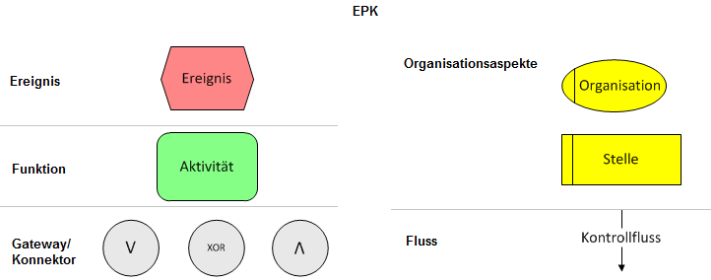
\includegraphics[width=13cm]{images/epk.png}
\caption{
EPK-Elemente
\newline
}
}
\end{center}
\end{minipage}
\end{figure}


Ein Ereignis repräsentiert sowohl einen Ausgangs- als auch einen Endpunkt.
Dieses bestimmt auch welche Zustände bzw. welche Bedingungen einen Prozess
auslösen und welche Zustände die Beendigung eines Prozesses definieren.

\subsubsection{BPMN}

Aus der folgenden Grafik kann man entnehmen, dass BPMN auf sehr ähnliche
Notationselemente zurückgreift, jedoch fordert es nicht nur
fachliche Prozessdokumentation, sondern auch informationstechnologische
Konventionen zu berücksichtigen.

\begin{figure}[H]
\begin{minipage}{\linewidth}
\begin{center}
\fbox{
\centering
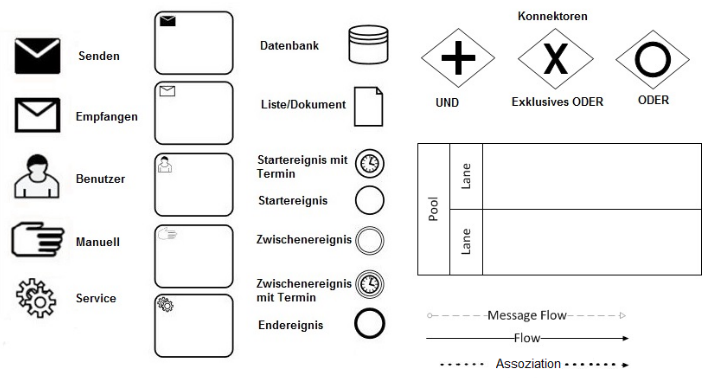
\includegraphics[width=13cm]{images/bpmn.png}
\caption{
BPMN-Elemente
\newline
}
}
\end{center}
\end{minipage}
\end{figure}

Die BPMN-Elemente werden insgesamt in fünf Kategorien eingeteilt: Flussobjekte
(Aktivitäten, Senden, Empfangen etc.), Verbindende Objekte
(Message Flow, Flow, Assoziation etc.), Daten (Datenobjekt, Liste, Dokument etc.),
Swimlanes (Pool, Lanes) und Artefakte (Gruppierungen, Anmerkungen etc.).

Ein Prozess wird häufig für eine (juristisch) selbstständige  Geschäftseinheit
(Business Unit) oder Organisation modelliert. Eine solche Geschäftseinheit
kann Teilnehmer (participant) an einer Zusammenarbeit zwischen zwei,
oder mehreren Geschäftspartnern sein. Der "`Pool"'  dient als grafische
Darstellung einer selbstständigen Business Unit bzw. eines Teilnehmers
an einer Zusammenarbeit. Die Lanes darunter können als sogenannte "`Schwimmbahnen"'
Swimlanes gesehen werden. Diese können untergeordnete Partnerrollen
(z.B. Vertrieb, Projektleitung, Beschaffung, Bereich) oder Komponenten
eines Systems sein und sie zeigen für welche Aktivitäten sie verantwortlich sind.
Der Pool ist den Lanes übergeordnet und enthält die Lanes.\\

Ein Prozess startet und endet in der Regel mit einem Ereignis (Startereignis
bzw. Endereignis). BPMN schreibt nicht zwingend vor, wie und ob Start-
und Endereignisse zu modellieren sind, es hilft jedoch zum besseren Verständnis.
Ereignisse werden durch einen Kreis dargestellt, je nach Art- eine schmale
unterbrochene, oder eine dicke durchgezogene Kreislinie- gekennzeichnet.
Die Aktivitäten können als Kern eines Prozesses verstanden werden.
Sie stellen ein Rechteck mit abgerundeten Ecken dar und werden am
sinnvollsten mit einer „Objekt+Verb“-Verbindung (z.B Verfügbarkeit prüfen)
beschriftet. Gateways dagegen sind als Kontrolle, Steuerung von Prozessen
und als Verbindung zwischen Aktivitäten zu verstehen. Für diese wird die
Raute als Zeichen verwendet, welches je nachdem, welche Entscheidungsmöglichkeit
es gibt, mit einem X, einem XOR oder einem OR beschriftet wird.\\

In welcher Reihenfolge die vorgenannten Elemente durchlaufen werden bestimmen
die "`Sequenzflüsse"' (sequence flow). Es handelt sich hierbei um einen
durchgängigen Verbindungspfeil mit "`ausgefüllter"' Spitze, welches jedoch nur
innerhalb eines Pools, auch Lane-übergreifend, verwendet werden kann.
Der Austausch zwischen den Pools dagegen geschieht durch "`Nachrichtenflüsse"' (message flows),
 welche durch einen "`gestrichelten"' Verbindungspfeil mit leerer Spitze gekennzeichnet
 sind. Hierbei sind noch einige Regeln zu beachten: Nachrichtenflüsse können nur mit
 sendenden oder empfangenden Nachrichten-Ereignissen verbunden werden.
 Nachrichtenflüsse dürfen zudem nicht in ein Nachrichten-Ereignis hinein- und
 gleichzeitig wieder herausführen, da jedes Nachrichten-Ereignis entweder sendend
 oder empfangend ist und nicht gleichzeitig beides.\\


In der Praxis kommen häufig komplexe Prozessmodelle vor.
Um die Brücke zwischen Business und IT zu schlagen,
können mit Hilfe von BPMN Geschäftsprozesse verständlicher und ausführbar
beschrieben und entworfen werden.\\



\subsection{Vorgehen bei der Modellierung}
Im folgenden wird beschrieben wie ein Prozess modelliert und anschließend
automatisiert werden kann. Hierzu wird BPMN in Verbindung mit dem Produkt
Bonita-Soft verwendet.

\subsubsection{Erstellung des Prozessmodell}

\paragraph{Subject-Prädikat-Objekt-Analyse} ist ein Vorgehensmodell das sich
sehr stark an die Grammatik der deutschen Sprache anlehnt. Dabei wird der
Prozess, welcher in Textform vorliegt, in seine Grundbausteine aufgeteilt um so
das vollständige Verständnis zu gewährleisten. Aufgeteilt wird in die 3
Bausteine:

\begin{itemize}
\item Subjekt - Wer oder was?
\item Prädikat - Was macht das Subjekt?
\item Objekt - Wen oder was?
\end{itemize}



\subsubsection{Automatisierung des Workflow}

Der folgende Prozess zur Bestellung eines Stiftes wurde modelliert:


\begin{figure}[H]
\begin{minipage}{\linewidth}
\begin{center}
\fbox{
\centering
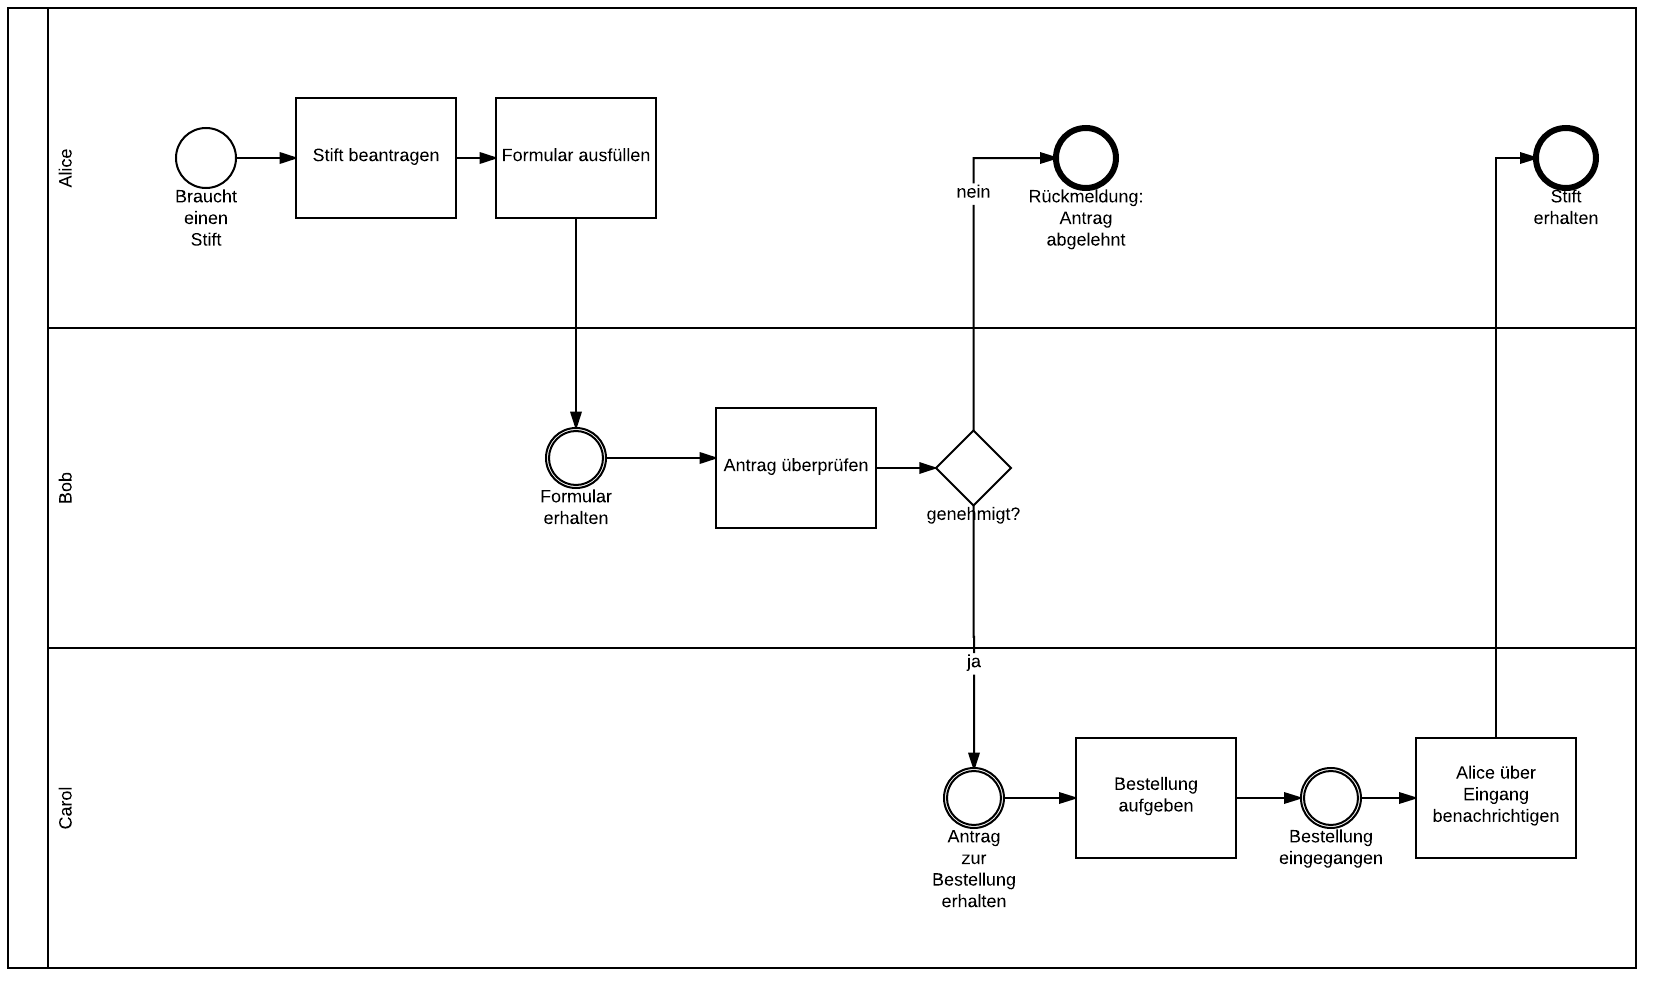
\includegraphics[width=13cm]{images/sampleprocess.png}
\caption{
Beispiel Prozess
\newline
}
}
\end{center}
\end{minipage}
\end{figure}


Mitarbeiterin Alice benötigt einen Stift und befolgt alle dazu nötigen
Arbeitsschritte. Dazu füllt sie das Formular in Papierform aus und bringt es
Bob, der für die Genehmigung zuständig ist. Das Formular bleibt bei Bob erst
einmal auf dem Schreibtisch liegen, bis dieser das Papier entdeckt und absegnet.
Nun leitet er es an Carol im Einkauf weiter, die den Stift nun bestellt. Beim
Wareneingang kontaktiert sie Alice, die nun den Stift abholen kann.
\\
\\
Der Prozess wäre wesentlich effizienter, wenn
\begin{enumerate}
  \item Alice ein Webformular ausfüllen würde
  \item Bob den Antrag mit einem weiteren Formular
bestätigen könnte
\item Carol eine Aufgabe zur Bestellung erhalten würde
\item und Carol Alice automatisch nach Ankunft der Bestellung benachrichtigen
könnte.
\end{enumerate}

Prozesse zu Modellieren und anschließend zu automatisieren hat diverse Vorteile:

\begin{enumerate}
\item Weniger Bürokratie
\item Verkürzung der Prozessdauer
\item Qualitätssteigerung
\item Standards und Konformität in der Ausführung und im Endprodukt
\footcite{automatisierungspros}
\end{enumerate}

Mit Hilfe von Software, wie z.B. Bonita BPM, lassen sich Geschäftsprozesse
automatisieren. So kann jeder Prozessbeteiligte ein Konto
besitzen, in dem er eine Übersicht aller offenen Aufgaben und
Zugriffe auf die Workflows hat.

Beispielsweise können Events, wie der Eingang einer Nachricht in einer Taskliste
erscheinen.

\begin{figure}[H]
\begin{minipage}{\linewidth}
\begin{center}
\fbox{
\centering
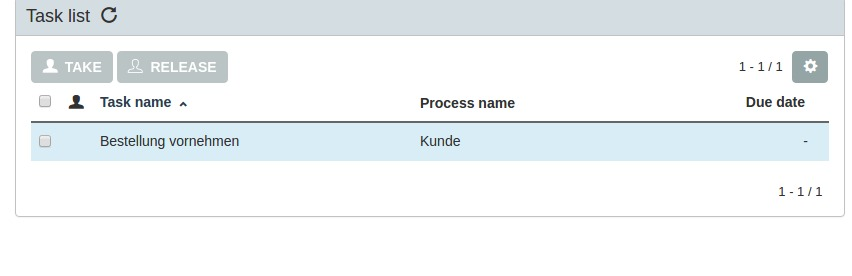
\includegraphics[width=13cm]{images/taskliste.jpeg}
\caption{
Beispiel; Taskliste in Bonita BPM
\newline
}
}
\end{center}
\end{minipage}
\end{figure}


Anstatt Formulare auf Papieren auszudrucken, können Formulare mit wenigen
Mausklicks zusammengestellt werden.

\begin{figure}[H]
\begin{minipage}{\linewidth}
\begin{center}
\fbox{
\centering
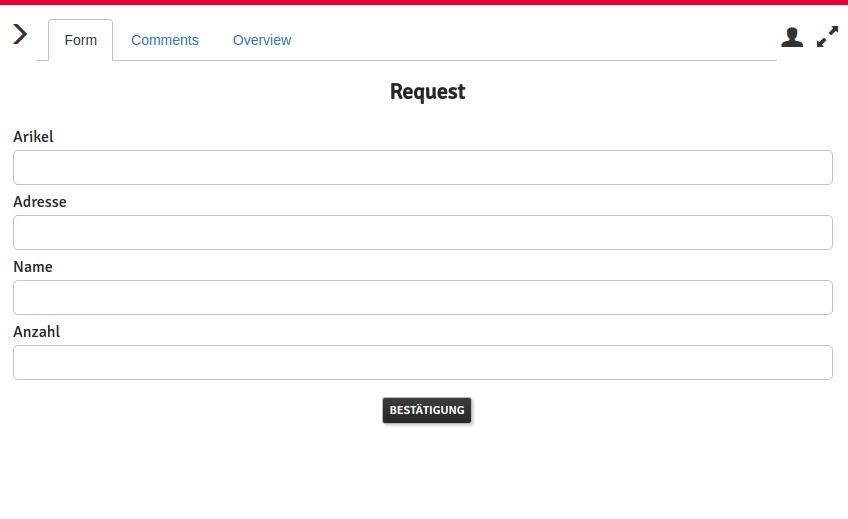
\includegraphics[width=13cm]{images/formular.jpeg}
\caption{
Beispiel: Formular in Bonita BPM
\newline
}
}
\end{center}
\end{minipage}
\end{figure}

Der Vorteil solcher BPM-Software wie Bonita ist, dass Prozesse ohne Entwickler
automatisiert werden.  Im Folgenden werden solche Anwendungen vorgestellt.


\clearpage
\section{Software für BPM}

Wie bereits im vorangegangenen Beispiel erläutert, ist es um so wichtiger,
Prozessmanagement durch IT zu unterstützen.

Im Laufe der Zeit haben sich immer mehr Anbieter am Markt etabliert,
die Lösungen zur Modellierung und Automatisierung von BPM anbieten. Allein in
der Wikipedia-List befindet sich eine Auflistung von 25 Unternehmen.\footcite{wikitools} Im
Folgenden werden ein paar Systeme vorgestellt und verglichen.

\subsection{ARIS Express}

\begin{figure}[H]
\begin{minipage}{\linewidth}
\begin{center}
\fbox{
\centering
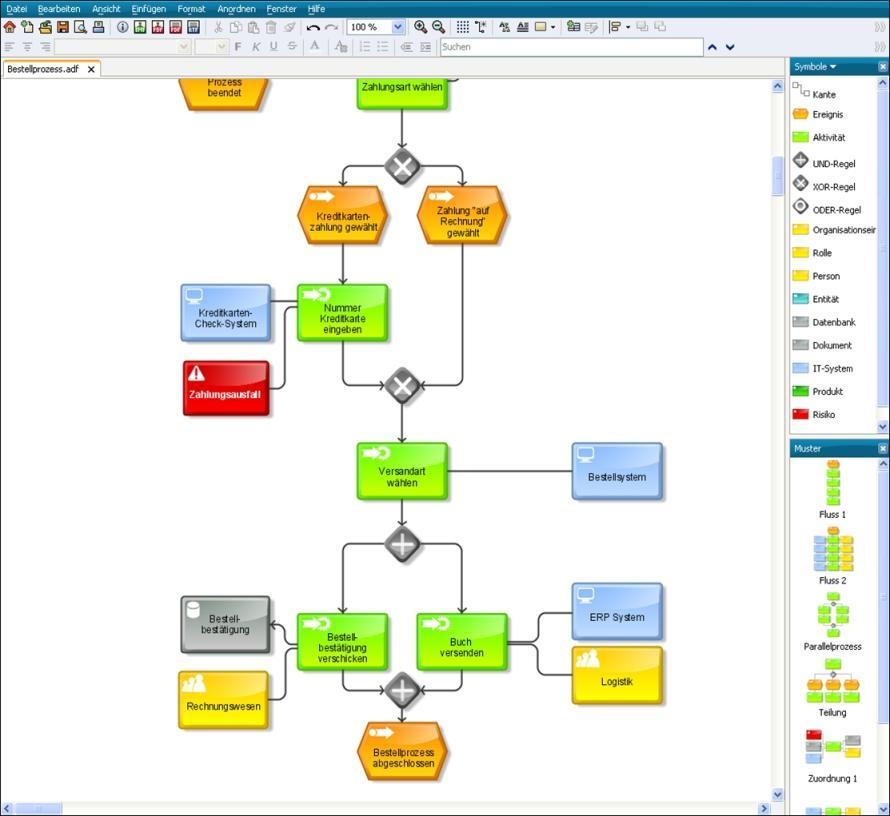
\includegraphics[width=13cm]{images/aris.jpg}
\caption{
Screenshot von ARIS Express
\newline
Quelle: {\protect\url{
https://www.computerwoche.de/i/detail/artikel/1928049/1/940760/d2e73-media/
}}\newline
Aufruf: 13.12.2017
}
}
\end{center}
\end{minipage}
\end{figure}

ARIS Express wird von der Darmstädter Software AG seit 2009 entwickelt und
vertrieben. Die Software wird als "`freeware"' vertrieben wodurch die
grundsätzliche Nutzung kostenfrei ist.
\\

ARIS läuft dabei als Java-Applikation
auf dem Rechner des Nutzers wodurch es möglich ist, das Tool sowohl auf Windows-
als auch auf Linux- und Mac-Betriebssystemen zu nutzen.
Hierbei ist neben BPMN 2.0 auch die Nutzung von eventgetriebenen
Prozessketten (EPC), Organisationsdiagrammen,
Prozesslandschaften und Whiteboards möglich.\\

Beachtenswert ist vor allem das intuitive Bedienungskonzept.
Auch ohne Einführung und Vorkentnisse ist es dem Nutzer bereits möglich einfache
Prozessketten abzubilden.





\subsection{Bonita BPM}

Bonita ist eine Open-Source-Software welche seit 2001 entwickelt wird. Der
Quellcode ist dabei via Github unter der GNU-Lizenz einseh- und
änderbar.\footcite{bonitasource}

\begin{figure}[H]
\begin{minipage}{\linewidth}
\begin{center}
\fbox{
\centering
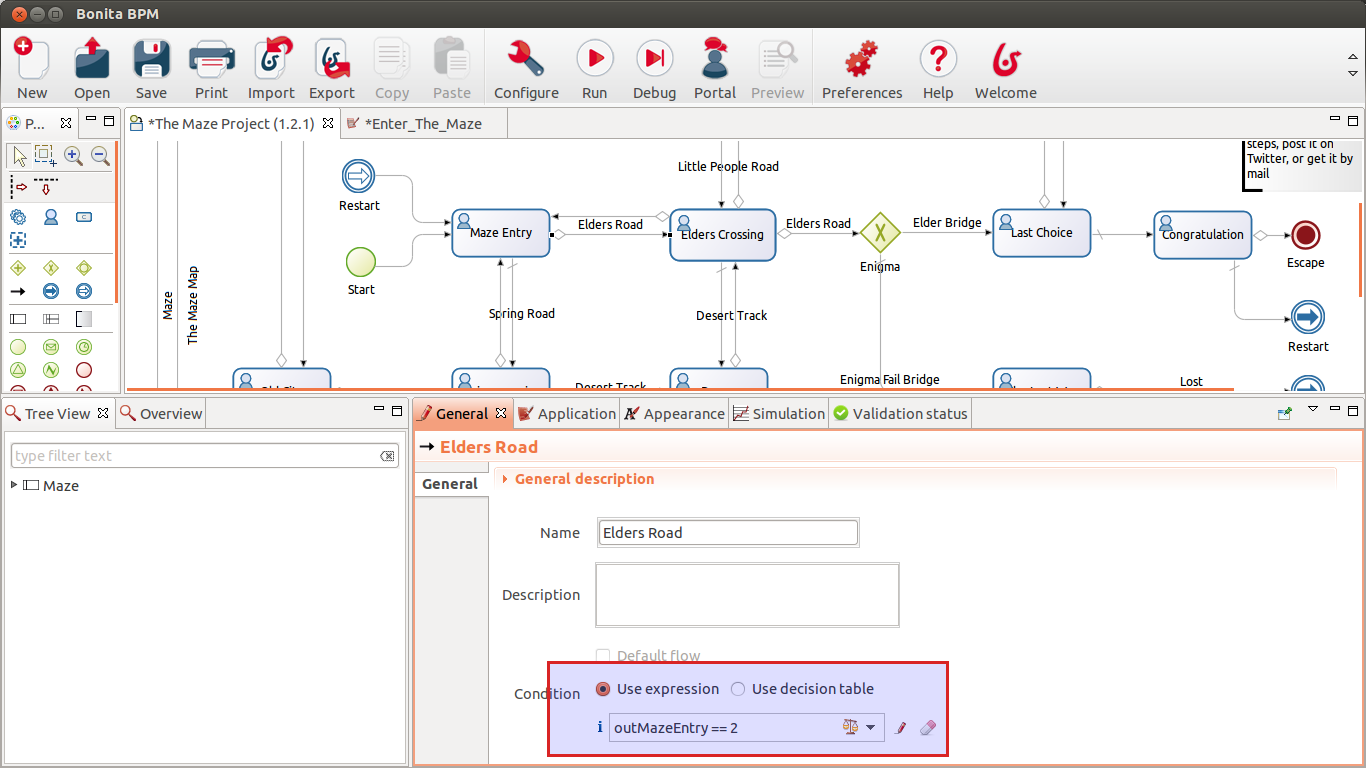
\includegraphics[width=14cm]{images/bonita.png}
\caption{
Screenshot von Bonita BPM
\newline
Quelle: {\protect\url{
http://i.imgur.com/ZY46h1R.png
}}\newline
Aufruf: 13.12.2017
}
}
\end{center}
\end{minipage}
\end{figure}

Bonita ist ebenfall, wie ARIS Express, eine Java-Anwendung wodurch sie auf allen
gängigen Betriebssystemen eingesetzt werden kann.

Über die Bonita Community erhält man Zugriff auf Foren und Video-Tutorials, die
den Einstieg vereinfachen. \footcite{bonitalernen}

\subsection{Bizagi}

Bizagi verspricht eine einfache und intuitive Prozessmodellierung.
Bizagi BPM kann entweder on-premise oder in der Cloud gehostet werden.
Über Cloud-Funktionen können von Chat- oder auch Teilfunktionen
profitiert werden. \footcite{bizagi} Darüber hinaus verspricht Bizagi ein
mobile-first und intuitives User Interface, dass die Nutzung über alle Geräte
hinweg unstertützt. \footcite{bizagimobile}


\begin{figure}[H]
\begin{minipage}{\linewidth}
\begin{center}
\fbox{
\centering
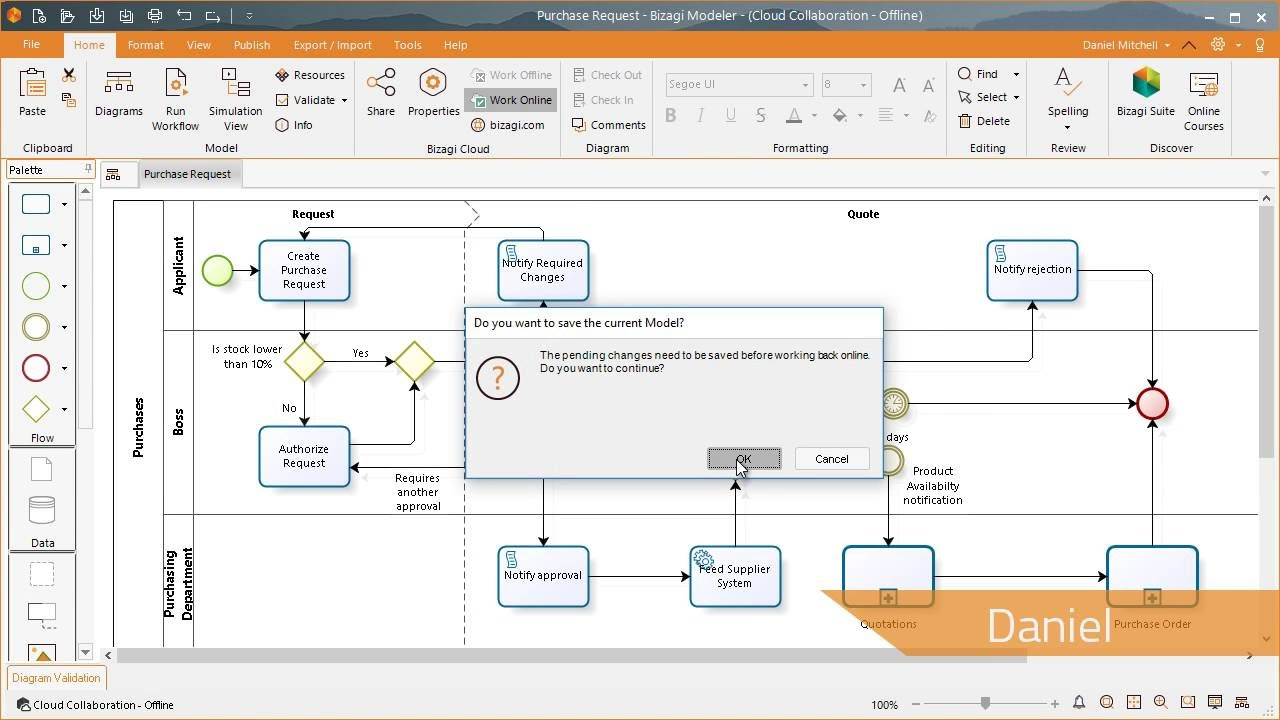
\includegraphics[width=14cm]{images/bizagi.jpg}
\caption{
Screenshot von Bizagi
\newline
Quelle: {\protect\url{
https://i.ytimg.com/vi/GfuEZaY7CvQ/maxresdefault.jpg
}}\newline
Aufruf: 15.12.2017
}
}
\end{center}
\end{minipage}
\end{figure}

Bizagi ist keine kostenfreie Lösung. Je nach Hosting - on-premise oder Cloud,
variiert das Lizenzmodell. Während on-premise pro Nutzer und für die Wartung
abgerechnet wird, sind die Kosten in der Cloud Nutzungsbasiert. Nutzungsbasiert
bedeutet, dass nur dann Kosten entstehen, wenn etwas genutzt wird.
\footcite{bizagipricing} Leider wird nicht ganz ersichtlich, wie diese Kosten in
Relation zum Nutzen entstehen.

Ein großer Vorteil von Bizagi ist, dass viele gratis, self-service
Trainingskurse angeboten werden. \footcite{bizagiproscons}
\footcite{bizagilernen}


\subsection{Ergebnis}

Die drei Anwendungen ARIS Express, Bonita BPM und Lucidchart werden nun
miteinander aufgrund von unterschiedlichen Parametern verglichen.
\\
\\
\textbf{Hosting} ARIS Express und Bonita BPM müssen beide lokal installiert
werden. Da Bizagi in der Cloud gehostet werden kann, ist der
Implementierungsaufwand geringer.
\\
\\
\textbf{Preismodell} ARIS Express basiert  auf dem Freemium
Modell, d.h. es besitzt eine kostenlose Grundversion. Bonita BPM ist eine Open
Source Software und somit frei und gratis zugänglich. \footcite{bonitasource}
Wenn Bizagi on-premise gehostet wird, dann fällt eine Lizenz pro User von 730 Euro an, zuzüglich
Wartungskosten von ca. 150 Euro. Eine Nutzungsbasierte Lizenz fällt bei der
Cloud-Version an. \footcite{bizagiprizing}
\\
\\
\textbf{Benutzerfreundlichkeit} Alle Anwendungen haben eine gute
Benutzerfreundlichkeit, Bizagi und Bonita BPM heben sich jedoch durch ein
moderneres Design ab.
\\
\\
\textbf{Mobile Unterstützung} Alle Systeme, außer ARIS, unterstützen mobile
Endgeräte.
\\
\\
\textbf{Lernen} Bizagi hebt sich vor allem durch die vielen angebotetenen Kurse
und Zertifizierungen ab. Bonitasoft bietet dagegen eine Community mit Foren und
Video Tutorials.

\begin{figure}[H]
\begin{minipage}{\linewidth}
\begin{center}
\fbox{
\centering
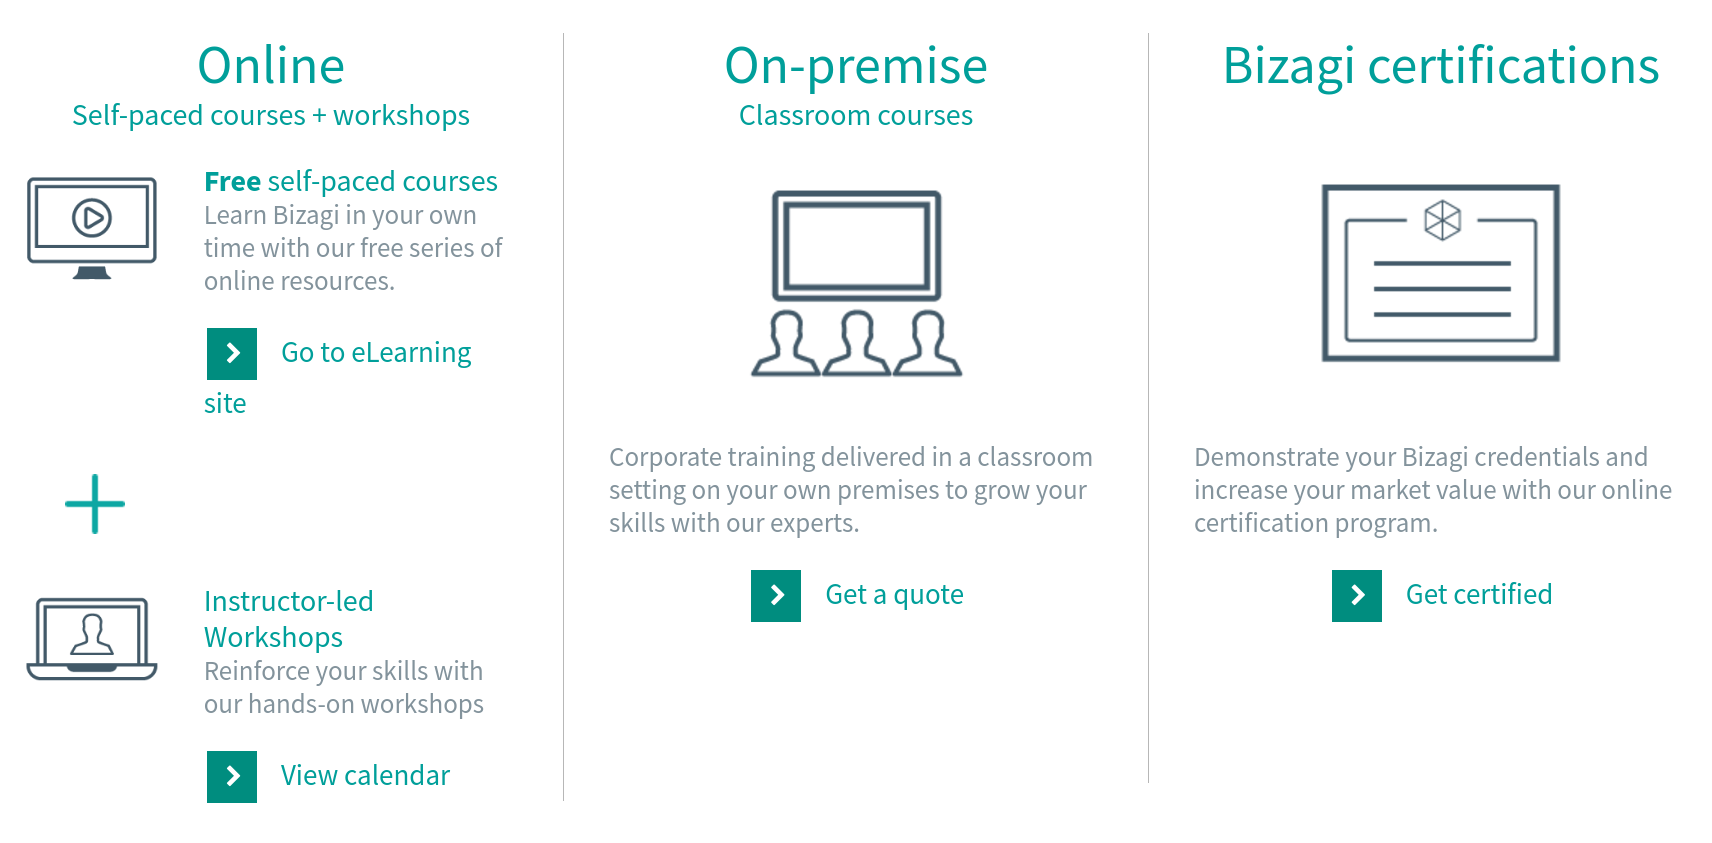
\includegraphics[width=10cm]{images/bizagikurse.png}
\caption{
Screenshot von Bizagis Kursen und Zertifizierungen
\newline
Quelle: {\protect\url{
https://www.bizagi.com/en/learning
}}\newline
Aufruf: 15.12.2017
}
}
\end{center}
\end{minipage}
\end{figure}
\\
\\
\textbf{Import} Dokumentation zu den Import- und Exportformaten lässt sich zu
ARIS Express nicht finden. Während in Bizagi der Import von Visio, XPDL oder
auch BPMN möglich ist,\footcite{bizagiimport} unterstützt Bonita BPM darüber
hinaus auch Formate von anderen BPM-Tools, wie z.B. ARIS.
\footcite{bonitaimportexport}
\\
\\
\textbf{Export} Bonita BPM exportiert Diagramme in gängige Bildformate.
\footcite{bonitaimportexport} Bizagi punktet mit einer Vielzahl an
Exportmöglichkeiten: Word, PDF, Excel oder auch Visio.
\footcite{bizagiexport}

\begin{figure}[H]
\begin{minipage}{\linewidth}
\begin{center}
\fbox{
\centering
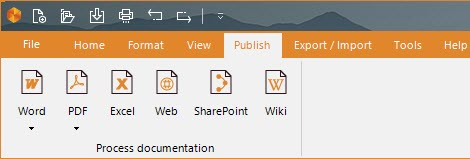
\includegraphics[width=14cm]{images/bizagiexport.jpg}
\caption{
Screenshot von Bizagis Export Funktionen
\newline
Quelle: {\protect\url{
http://help.bizagi.com/process-modeler/en/generating1.jpg
}}\newline
Aufruf: 15.12.2017
}
}
\end{center}
\end{minipage}
\end{figure}

\\
\\

\begin{table}[h]
\begin{tabularx}{\textwidth}{|X|c|c|c|c|}
	\hline
	\textbf{Parameter}  & \textbf{ARIS Express} &
	\textbf{Bonita BPM} & \textbf{Lucidchart}  \\
	\hline
	\hline
	\textbf{Hosting} & {Lokal (Java)} & {Lokal (Java)} 3 & {On-Premise/Cloud}
	\\
	\hline
	\textbf{Preismodell} & Freemium & Open Source &  kostenpflichtig\\
	\hline
	\textbf{Usability} & gut & sehr gut & sehr gut \\
	\hline
	\textbf{Import} & -* & sehr gut & gut \\
	\hline
	\textbf{Export} & -* & gut & sehr gut \\
	\hline
	\textbf{Mobile Support} & nein & ja & ja \\
	\hline
\end{tabularx}
\caption{Vergleich von BPMN-Modellierungssoftware}
\end{table}
* Informationen nicht bekannt.
\\
\\
Die Analyse ergibt, dass Bonita BPM und Bizagi deutlich
besser in den Kategorien abschneiden als ARIS Express. Bonita BPM und Bizagi
sind wesentlich benutzerfreundlicher und unterstützen mobile
Endgeräte. Bizagi punktet vor allem durch die diversen Exportmöglichkeiten, während Bonita BPM mehr Importformate anbietet und ihre
Software Open Source zur Verfügung stellt.

\clearpage
\section{Fazit}

Mit der hier vorliegenden Arbeit wurde gezeigt wie wichtig die
Geschäftsprozessmodellierung mittlerweile im Unternehmensumfeld geworden ist.
Neben der Quasi-Standardlösung BPMN gibt es dabei noch weitere
Modellierungsformen wie EPK.\\
Zu dem gibt es eine ganze Reihe von Softwareprodukten welche zar ähnliche
Grundfunktionen besitzen, sich in den Feinheiten jedoch stark unterscheiden.
Dadurch ist es sowhol wichtig mehrere Produkte zu kennen, sowie die Auswahl
 mit Bedacht zu treffen.


\clearpage
